\section{Casi d'uso}
\subsection{Scopo}
L'obbiettivo di questa sezione è quello di presentare e descrivere tutti i casi d'uso, individuati dal team, in riferimento alle funzionalità richieste nell'applicazione.
\subsection{Attori}
Non essendo richiesto nessun tipo di servizio di autenticazione o più in generale una distinzione gerarchica degli utenti, è presente un solo attore nella gerarchia ovvero: l'utente generico.
\begin{figure}[h!]
    \centering
    
\includegraphics[scale=0.50]{../../assets/Utente.png}
    \caption{Gerarchia attori}
\end{figure}

% --------------------------------------------------------------------
% INIZIO CASI D'USO
% CARICAMENTO DATASET
% --------------------------------------------------------------------

\subsection{UC1 - Caricamento dataset}
\begin{figure}[h!]
    \centering
    % Sistema immagine inserendo tag UC e abbelliscila dc
    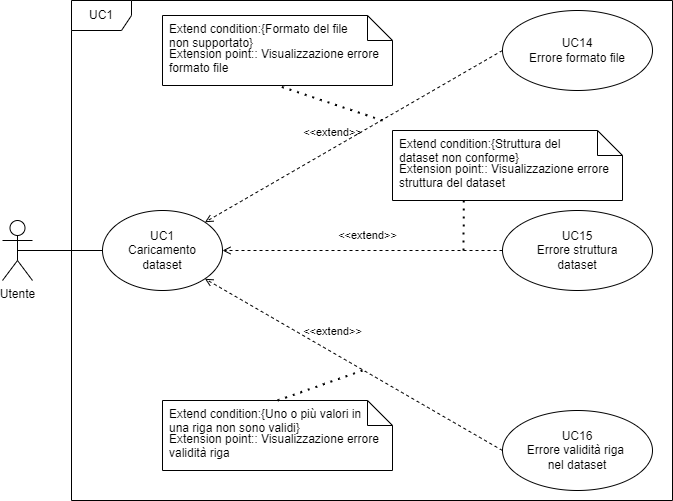
\includegraphics[scale=0.60]{../../assets/Caricamento_dataset.png}
    \caption{UC1 - Caricamento ${\mathrm{dataset^{G}}}$}
\end{figure}
\begin{itemize}
    \item \textbf{Attore primario:} Utente.
    \item \textbf{Precondizioni:} Il sistema è funzionante
    \item \textbf{Postcondizioni:} Viene visualizzato un messaggio che avvisa l'utente del corretto caricamento dei dati e della loro validità. 
                                   I dati vengono caricati nel sistema
    \item \textbf{Scenario principale:}
          \begin{enumerate}
              \item L'utente seleziona il file da caricare
              \item L'utente carica il file
          \end{enumerate}
    \item \textbf{Estensioni:}
    \begin{itemize}
        \item   Nel caso in cui l'utente carichi un file in un formato non supportato
                \begin{enumerate}
                    \item I dati non vengono caricati
                    \item Viene visualizzato un messaggio di errore esplicativo [\hyperref[sec:UC14 - Errore formato file]{UC14}] % To Do: metti il link alla sezione   
                \end{enumerate}
        \item   Nel caso in cui l'utente carichi un file non correttamente strutturato
                \begin{enumerate}
                    \item I dati non vengono caricati
                    \item Viene visualizzato un messaggio di errore esplicativo [\hyperref[sec:UC15 - Errore struttura dataset]{UC15}]
                \end{enumerate}
        \item   Nel caso in cui i dati di una o più righe non siano validi
                \begin{enumerate}
                    \item Viene visualizzato un messaggio di errore esplicativo [\hyperref[sec:UC16 - Errore validità riga]{UC16}] 
                \end{enumerate}
    \end{itemize} 
\end{itemize}
\newpage

% --------------------------------------------------------------------
% SCELTA TIPO GRAFICO
% --------------------------------------------------------------------

\subsection{UC2 - Scelta tipologia grafico}
\label{sec:UC2}
\begin{figure}[h!]
    \centering
    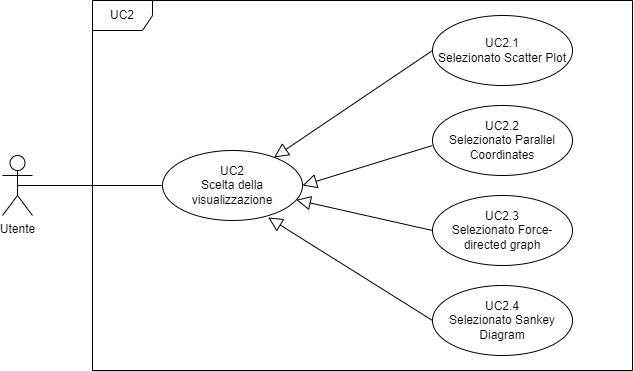
\includegraphics[scale=0.60]{../../assets/Selezione_tipo_grafico.png}
    \caption{UC2 - Scelta tipologia grafico}
\end{figure}
\begin{itemize}
    \item \textbf{Attore primario}: Utente.
    \item \textbf{Precondizioni}: Il ${\mathrm{dataset^{G}}}$ è stato caricato correttamente.
    \item \textbf{Postcondizioni}: Viene mostrata la visualizzazione scelta.
    \item \textbf{Scenario principale}:
          \begin{enumerate}
              \item L'utente seleziona il tipo di grafico da visualizzare tra le tipologie disponibili.
          \end{enumerate}
    \item \textbf{Generalizzazioni}:
    \begin{itemize}
        \item L'utente seleziona una delle seguenti opzioni:
                \begin{enumerate}
                    \item \textit{$Scatter$ $Plot^{G}$} \hyperref[sec:UC2.1]{UC2.1}.
                    \item \textit{$Parallel$ $Coordinates^{G}$} \hyperref[sec:UC2.2]{UC2.2}.
                    \item \textit{$Force-directed$ $Graph^{G}$} \hyperref[sec:UC2.3]{UC2.3}.
                    \item \textit{$Sankey$ $Diagram^{G}$} \hyperref[sec:UC2.4]{UC2.4}.
                \end{enumerate}
    \end{itemize} 
\end{itemize}

\subsubsection{UC2.1 - Selezione Scatter Plot}
\label{sec:UC2.1}
\begin{itemize}
    \item \textbf{Attore primario}: Utente.
    \item \textbf{Precondizioni}: Il ${\mathrm{dataset^{G}}}$ è stato caricato correttamente [UC2].
    \item \textbf{Postcondizioni}: Viene mostrata la visualizzazione $Scatter$ $Plot^{G}$ scelta dall'utente con possibilità di selezionare una diversa vista$^{G}$ \hyperref[sec:UC3]{UC3} e personalizzare grafico e stile \hyperref[sec:UC5.1]{UC5.1}. %inserire il numero corretto dello stile e delle dimensioni
    \item \textbf{Scenario principale}:
          \begin{enumerate}
              \item L'utente seleziona il grafico $Scatter$ $Plot^{G}$ e il sistema ritorna tale grafico con conseguente possibilità di personalizzazione. 
          \end{enumerate}
\end{itemize}

\subsubsection{UC2.2 - Selezione Parallel Coordinates}
\label{sec:UC2.2}
\begin{itemize}
    \item \textbf{Attore primario}: Utente.
    \item \textbf{Precondizioni}: Il ${\mathrm{dataset^{G}}}$ è stato caricato correttamente [UC2].
    \item \textbf{Postcondizioni}: Viene mostrata la visualizzazione $Parallel$ $Coordinates^{G}$ scelta dall'utente con possibilità di selezionare una diversa vista$^{G}$ \hyperref[sec:UC3]{UC3} e personalizzare grafico e stile \hyperref[sec:UC5.2]{UC5.2}. %inserire il numero corretto dello stile e delle dimensioni
    \item \textbf{Scenario principale}:
          \begin{enumerate}
              \item L'utente seleziona il grafico $Parallel$ $Coordinates^{G}$ e il sistema ritorna tale grafico con conseguente possibilità di personalizzazione. 
          \end{enumerate}
\end{itemize}

\subsubsection{UC2.3 - Selezione Force-directed Graph}
\label{sec:UC2.3}
\begin{itemize}
    \item \textbf{Attore primario}: Utente.
    \item \textbf{Precondizioni}: Il ${\mathrm{dataset^{G}}}$ è stato caricato correttamente [UC2].
    \item \textbf{Postcondizioni}: Viene mostrata la visualizzazione $Force-directed$ $Graph^{G}$ scelta dall'utente con possibilità di selezionare una diversa vista$^{G}$ \hyperref[sec:UC3]{UC3} e personalizzare grafico e stile \hyperref[sec:UC5.3]{UC5.3}. %inserire il numero corretto dello stile e delle dimensioni
    \item \textbf{Scenario principale}:
          \begin{enumerate}
              \item L'utente seleziona il grafico $Force-directed$ $Graph^{G}$ e il sistema ritorna tale grafico con conseguente possibilità di personalizzazione. 
          \end{enumerate}
\end{itemize}

\subsubsection{UC2.4 - Selezione Sankey Diagram}
\label{sec:UC2.4}
\begin{itemize}
    \item \textbf{Attore primario}: Utente.
    \item \textbf{Precondizioni}: Il ${\mathrm{dataset^{G}}}$ è stato caricato correttamente [UC2].
    \item \textbf{Postcondizioni}: Viene mostrata la visualizzazione $Sankey$ $Diagram^{G}$ scelta dall'utente con possibilità di selezionare una diversa vista$^{G}$ \hyperref[sec:UC3]{UC3} e personalizzare grafico e stile \hyperref[sec:UC5.4]{UC5.4}. %inserire il numero corretto dello stile e delle dimensioni
    \item \textbf{Scenario principale}:
          \begin{enumerate}
              \item L'utente seleziona il grafico $Sankey$ $Diagram^{G}$ e il sistema ritorna tale grafico con conseguente possibilità di personalizzazione. 
          \end{enumerate}
\end{itemize}
\newpage

%               _ _              _       _                 _
%  ___  ___ ___| | |_ __ _    __| | __ _| |_ __ _ ___  ___| |_
% / __|/ __/ _ \ | __/ _` |  / _` |/ _` | __/ _` / __|/ _ \ __|
% \__ \ (_|  __/ | || (_| | | (_| | (_| | || (_| \__ \  __/ |_
% |___/\___\___|_|\__\__,_|  \__,_|\__,_|\__\__,_|___/\___|\__|


\subsection{UC3 - Eliminazione Vista}
\label{sec:UC3}
\begin{figure}[h!]
    \centering
    % Controlla che UC abbia il numero corretto
    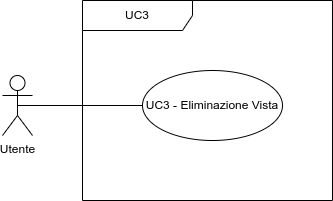
\includegraphics[scale=0.60]{../../assets/eliminazione_vista.png}
    \caption{UC3 - Eliminazione di una vista$^{G}$}
\end{figure}
\begin{itemize}
    \item \textbf{Attore primario}: Utente.
    \item \textbf{Precondizioni}: L'utente sta visualizzando una vista$^{G}$.
    \item \textbf{Postcondizioni}: Viene eliminata la vista selezionata.
    \item \textbf{Scenario principale}:
          \begin{enumerate}
              \item L'utente preme il pulsante elimina vista$^{G}$.
              \item La vista$^{G}$ viene eliminata.
              \item L'utente viene riportato alla visualizzazione di default.
          \end{enumerate}
\end{itemize}

\subsubsection{UC3.1 - Visualizzazione messaggio di conferma eliminazione}
\label{sec:UC3.1}
\begin{itemize}
	\item \textbf{Attore primario:} Utente.
	\item \textbf{Precondizioni:} Il ${\mathrm{dataset^{G}}}$ è presente e caricato correttamente. L'utente ha cliccato il pulsante per l'eliminazione di una vista$^{G}$ \hyperref[sec:UC3]{UC3}.
	\item \textbf{Postcondizioni:} Viene eliminata la vista$^{G}$, oppure l'operazione viene annullata.
	\item \textbf{Scenario principale:}
		\begin{enumerate}
		\item Viene visualizzato un messaggio di conferma per l'eliminazione della vista$^{G}$.
		\item L'utente sceglie una delle due opzioni:
			\begin{itemize}
				\item L'utente vuole ripristinare eliminare la vista$^{G}$ e clicca ``Ok''
				\item L'utente vuole annullare l'operazione e clicca ``Annulla''
			\end{itemize}
		\end{enumerate}
\end{itemize}

\newpage

% --------------------------------------------------------------------
% VISUALIZZAZIONE DI DEFAULT DEI GRAFICI
% --------------------------------------------------------------------

\subsection{UC4 - Visualizzazione di default dei grafici}
\label{sec:UC4}
\begin{figure}[h!]
    \centering
    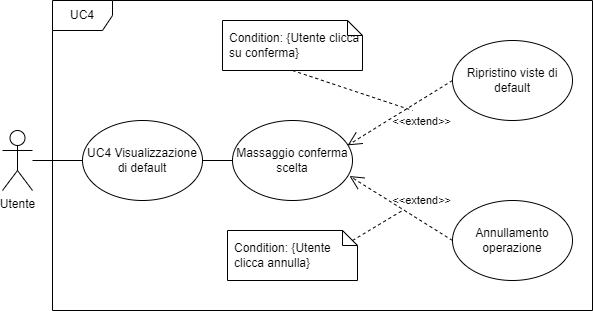
\includegraphics[scale=0.60]{../../assets/visualizzazione_default.png}
	\caption{UC4 - Visualizzazione di default dei grafici}
\end{figure}

\begin{itemize}
	\item \textbf{Attore primario:} Utente.
	\item \textbf{Precondizioni:} Il ${\mathrm{dataset^{G}}}$ è presente e caricato correttamente.
	\item \textbf{Postcondizioni:} Viene mostrato il messaggio relativo al ripristino delle impostazioni di default \hyperref[sec:UC4.1]{UC4.1}.
	\item \textbf{Scenario principale:}
	\begin{itemize}
		\item L'utente clicca sul pulsante ``Visualizzazione di default''.
		\item L'utente visualizza un messaggio di scelta.
	\end{itemize}
\end{itemize}

\subsubsection{UC4.1 - Visualizzazione messaggio di conferma scelta}
\label{sec:UC4.1}
\begin{itemize}
	\item \textbf{Attore primario:} Utente.
	\item \textbf{Precondizioni:} Il ${\mathrm{dataset^{G}}}$ è presente e caricato correttamente. L'utente ha cliccato il pulsante per il ripristino delle impostazioni di default \hyperref[sec:UC4]{UC4}.
	\item \textbf{Postcondizioni:} Viene ripristinato il grafico con le impostazioni di default, oppure l'operazione viene annullata.
	\item \textbf{Scenario principale:}
		\begin{enumerate}
		\item Viene visualizzato un messaggio di conferma per tornare alla visualizzazione di default del grafico.
		\item L'utente sceglie una delle due opzioni:
			\begin{itemize}
				\item L'utente vuole ripristinare le impostazioni di default e clicca ``Ok''
				\item L'utente vuole annullare l'operazione e clicca ``Annulla''
			\end{itemize}
		\end{enumerate}
\end{itemize}

\newpage

% --------------------------------------------------------------------
% SEZIONE PERSONALIZZAZIONE DEI GRAFICI
% --------------------------------------------------------------------

\subsection{UC5 - Personalizzazione dei grafici}
\begin{figure}[h!]
	\centering
	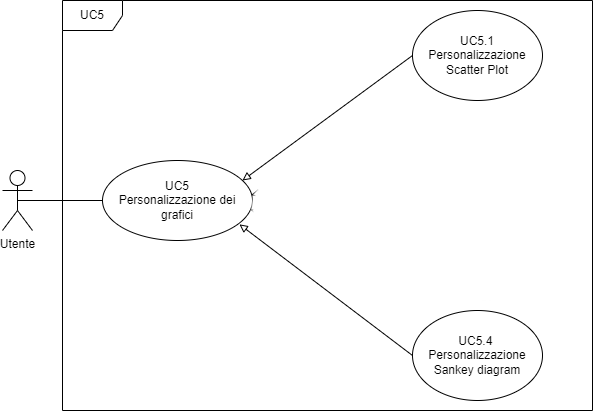
\includegraphics[scale=0.60]{../../assets/personalizzazioneVisivaGrafici.png}
	\caption{UC5 - Personalizzazione dei grafici}
\end{figure}
\begin{itemize}
	\item \textbf{Attore primario:} Utente.
	\item \textbf{Precondizioni:} L'utente ha scelto uno dei grafici a disposizione nell'interfaccia \hyperref[sec:UC2]{UC2}.
	\item \textbf{Postcondizioni:} Il grafico viene ridisegnato secondo le scelte selezionate dall'utente.
	\item \textbf{Scenario principale:}
	\begin{enumerate}
		\item Per ogni grafico l'utente ha a disposizione delle modifiche specifiche su: ${\mathrm{dimensione^{G}}}$, ordinamento e numero degli assi, scelta della funzione di forza, dell'algoritmo di integrazione, e ordinamento dei dati.
    		\item L'utente modifica anche lo stile del grafico.
    		\item Nel caso si scelga di tornare alla vista$^{G}$ di default, le modifiche eseguite torneranno ai valori standard.
    \end{enumerate}
    \item \textbf{Generalizzazioni}:
    \begin{itemize}
        \item L'utente seleziona una delle seguenti opzioni:
                \begin{enumerate}
                    \item \textit{Personalizza $Scatter$ $Plot^{G}$} \hyperref[sec:UC5.1]{UC5.1}.
                    \item \textit{Personalizza $Parallel$ $Coordinates^{G}$} \hyperref[sec:UC5.2]{UC5.2}.
                    \item \textit{Personalizza $Force-directed$ $Graph^{G}$} \hyperref[sec:UC5.3]{UC5.3}.
                    \item \textit{Personalizza $Sankey$ $Diagram^{G}$} \hyperref[sec:UC5.4]{UC5.4}.
                \end{enumerate}
    \end{itemize} 
\end{itemize}

% SCATTER PLOT
\newpage
\subsubsection{UC5.1 - Personalizzazione Scatter Plot}
\label{sec:UC5.1}
\begin{figure}[h!]
	\centering
	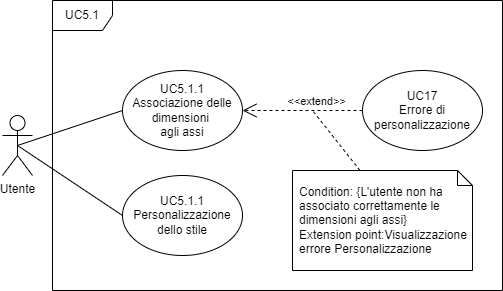
\includegraphics[scale=0.60]{../../assets/personalizzazioneScatterPlot.png}
	\caption{UC5.1 - Personalizzazione $Scatter$ $Plot^{G}$}
\end{figure}
\begin{itemize}
    \item \textbf{Attore primario:} Utente.
	\item \textbf{Precondizioni:} L'utente ha scelto il grafico $Scatter$ $Plot^{G}$. \hyperref[sec:UC2.1]{UC2.1}.
	\item \textbf{Postcondizioni:} 
	Il grafico viene ridisegnato secondo le scelte selezionate dall'utente.
	\item \textbf{Scenario principale:} L'utente decide:
	\begin{enumerate}
        \item Associazione delle ${\mathrm{dimensioni^{G}}}$ agli assi \hyperref[sec:UC5.1.1]{UC5.1.1}.
        \item Personalizzazione dello stile \hyperref[sec:UC5.1.2]{UC5.1.2}.
    \end{enumerate}
\end{itemize}
\paragraph{UC5.1.1 - Associazione delle dimensioni agli assi}
\label{sec:UC5.1.1}
    \begin{itemize}
        \item \textbf{Attore primario:} Utente.
        \item \textbf{Precondizioni:} L'utente ha selezionato il grafico $Scatter$ $Plot^{G}$ \hyperref[sec:UC2.1]{UC2.1}.
	    \item \textbf{Postcondizioni:} L'utente ha associato le ${\mathrm{dimensioni^{G}}}$ disponibili con gli assi del grafico.
	    \item \textbf{Scenario principale:} 
	    \begin{enumerate}
	    		\item L'utente sceglie quali ${\mathrm{dimensioni^{G}}}$ associare agli assi del grafico.
		\end{enumerate}
	    \item \textbf{Estensioni:} Nel caso l'utente non abbia associato correttamente le ${\mathrm{dimensioni^{G}}}$ agli assi del grafico:
              \begin{itemize}
                  \item Non viene visualizzato nessun grafico.
                  \item Viene visualizzato un errore di personalizzazione grafico \hyperref[sec:UC17 - Errore di personalizzazione]{UC17}.
              \end{itemize}
    \end{itemize}
\paragraph{UC5.1.2 - Personalizzazione dello stile}
\label{sec:UC5.1.2}
    \begin{itemize}
        \item \textbf{Attore primario:} Utente.
        \item \textbf{Precondizioni:} L'utente ha selezionato il grafico $Scatter$ $Plot^{G}$ \hyperref[sec:UC2.1]{UC2.1}.
	    \item \textbf{Postcondizioni:} L'utente ha associato nuovi colori ai punti.
	    \item \textbf{Scenario principale:} 
	    \begin{enumerate}
	    		\item L'utente visualizza le opzioni di colori per la personalizzazione di ogni specifica del grafico.
	    		\item Nel caso l'utente non li modifichi rimangono quelli di default.
		\end{enumerate}
    \end{itemize}

% PARALLEL CORDINATES 
\subsubsection{UC5.2 - Personalizzazione Parallel Coordinates}
\label{sec:UC5.2}
\begin{figure}[h!]
	\centering
	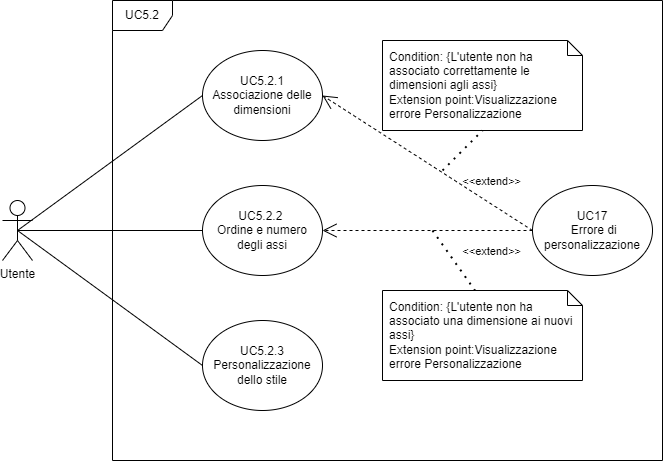
\includegraphics[scale=0.60]{../../assets/personalizzazioneParallelCoordinates.png}
	\caption{UC5.2 - Personalizzazione $Parallel$ $Coordinates^{G}$}
\end{figure}
\begin{itemize}
    \item \textbf{Attore primario:} Utente.
	\item \textbf{Precondizioni:} L'utente ha scelto il grafico $Parallel$ $Coordinates^{G}$ \hyperref[sec:UC2.2]{UC2.2}.
	\item \textbf{Postcondizioni:} Il grafico viene ridisegnato secondo le scelte selezionate dall'utente.
	\item \textbf{Scenario principale:} L'utente decide:
	\begin{enumerate}
        \item Associazione delle ${\mathrm{dimensioni^{G}}}$ \hyperref[sec:UC5.2.1]{UC5.2.1}.
        \item Ordine degli assi \hyperref[sec:UC5.2.2]{UC5.2.2}.
        \item \textit{Scaling} dei dati \hyperref[sec:UC5.2.3]{UC5.2.3}.
        \item Personalizzazione dello stile \hyperref[sec:UC5.2.4]{UC5.2.4}.
    \end{enumerate}
\end{itemize}

\paragraph{UC5.2.1 - Associazione delle dimensioni}
\label{sec:UC5.2.1}
    \begin{itemize}
        \item \textbf{Attore primario:} Utente.
        \item \textbf{Precondizioni:} L'utente ha selezionato $Parallel$ $Coordinates^{G}$ \hyperref[sec:UC2.2]{UC2.2}.
	    \item \textbf{Postcondizioni:} L'utente ha associato le ${\mathrm{dimensioni^{G}}}$ disponibili con gli assi del grafico.
	    \item \textbf{Scenario principale:}
	    \begin{enumerate}
	    		\item L'utente sceglie quali ${\mathrm{dimensioni^{G}}}$ associare agli assi del grafico.
		\end{enumerate}
	    \item \textbf{Estensioni:} Nel caso l'utente non abbia associato correttamente le ${\mathrm{dimensioni^{G}}}$ agli assi del grafico:
              \begin{itemize}
                  \item Non viene visualizzato nessun grafico.
                  \item Viene visualizzato un errore di personalizzazione grafico \hyperref[sec:UC17 - Errore di personalizzazione]{UC17}.
              \end{itemize}
    \end{itemize}
\paragraph{UC5.2.2 - Ordine e numero degli assi}
\label{sec:UC5.2.2}
    \begin{itemize}
        \item \textbf{Attore primario:} Utente.
        \item \textbf{Precondizioni:} L'utente ha selezionato $Parallel$ $Coordinates^{G}$ \hyperref[sec:UC2.2]{UC2.2}.
	    \item \textbf{Postcondizioni:} L'utente ha modificato l'ordine verticale degli assi e il numero, il grafico quindi riduce o aumenta gli intrecci paralleli.
	    \item \textbf{Scenario principale:} 
	    \begin{enumerate}
	    		\item L'utente sceglie ordine e numero degli assi.
		\end{enumerate}
	    \item \textbf{Estensioni:} Nel caso l'utente abbia creato nuovi assi ma non abbia associato nessuna ${\mathrm{dimensione^{G}}}$ a essi:
              \begin{itemize}
                  \item Non viene visualizzato nessun grafico.
                  \item Viene visualizzato un errore di personalizzazione grafico.
              \end{itemize}
    \end{itemize}
    
\paragraph{UC5.2.3 - Scaling dei dati}
\label{sec:UC5.2.3}
    \begin{itemize}
        \item \textbf{Attore primario:} Utente.
        \item \textbf{Precondizioni:} L'utente ha selezionato $Parallel$ $Coordinates^{G}$ \hyperref[sec:UC2.2]{UC2.2}.
	    \item \textbf{Postcondizioni:} L'utente ha ridimensionato i dati in una nuova scala comune tra le variabili o viceversa.
	    \item \textbf{Scenario principale:} 
	    \begin{enumerate}
	    		\item L'utente sceglie lo \textit{scaling} dei dati.
		\end{enumerate}
    \end{itemize}

\paragraph{UC5.2.4 - Personalizzazione dello stile}
\label{sec:UC5.2.4}
    \begin{itemize}
        \item \textbf{Attore primario:} Utente.
        \item \textbf{Precondizioni:} L'utente ha selezionato $Parallel$ $Coordinates^{G}$ \hyperref[sec:UC2.2]{UC2.2}.
	    \item \textbf{Postcondizioni:} L'utente ha evidenziato uno specifico gruppo di linee di interesse modificandone i colori.
	    \item \textbf{Scenario principale:} 
	    \begin{enumerate}
	    		\item L'utente visualizza le opzioni di colori per la personalizzazione
	    		\item Nel caso l'utente non li modifichi rimangono quelli di default.
		\end{enumerate}
    \end{itemize}


% FORCE-DIRECTED GRAPH 
\subsubsection{UC5.3 - Personalizzazione Force-directed Graph}
\label{sec:UC5.3}
\begin{figure}[h!]
	\centering
	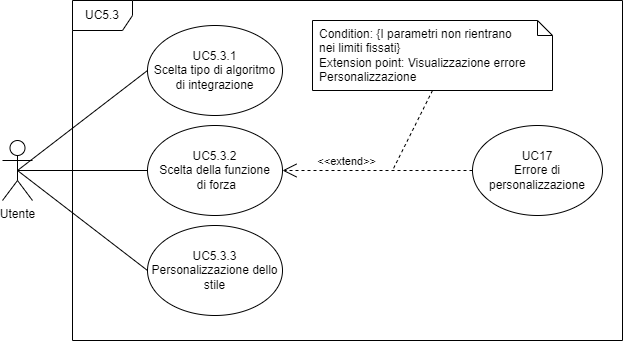
\includegraphics[scale=0.60]{../../assets/personalizzazioneForce-directedGraph.png}
	\caption{UC5.3 - Personalizzazione $Force-directed$ $Graph^{G}$}
\end{figure}
\begin{itemize}
    \item \textbf{Attore primario:} Utente.
	\item \textbf{Precondizioni:} L'utente ha scelto il grafico $Force-directed$ $Graph^{G}$ \hyperref[sec:UC2.3]{UC2.3}.
	\item \textbf{Postcondizioni:} Il grafico viene ridisegnato secondo le scelte selezionate dall'utente.
	\item \textbf{Scenario principale:}L'utente decide:
	\begin{enumerate}
        \item Scelta del tipo di algoritmo d'integrazione \hyperref[sec:UC5.3.1]{UC5.3.1}.
        \item Scelta della funzione di forza \hyperref[sec:UC5.3.2]{UC5.3.2}.
        \item Personalizzazione dello stile \hyperref[sec:UC5.3.3]{UC5.3.3}.
    \end{enumerate}
\end{itemize}
\paragraph{UC5.3.1 - Scelta tipo di algoritmo d'integrazione}
\label{sec:UC5.3.1}
    \begin{itemize}
        \item \textbf{Attore primario:} Utente.
        \item \textbf{Precondizioni:} L'utente ha selezionato $Force-directed$ $Graph^{G}$ \hyperref[sec:UC2.3]{UC2.3}.
	    \item \textbf{Postcondizioni:} L'utente ha scelto l'algoritmo d'integrazione che desidera.
	    \item \textbf{Scenario principale:}
	    \begin{enumerate}
	    		\item L'utente sceglie l'algoritmo d'integrazione che desidera.
		\end{enumerate}
    \end{itemize}
\paragraph{UC5.3.2 - Scelta della funzione di forza}
\label{sec:UC5.3.2}
    \begin{itemize}
        \item \textbf{Attore primario:} Utente.
        \item \textbf{Precondizioni:} L'utente ha selezionato $Force-directed$ $Graph^{G}$ \hyperref[sec:UC2.3]{UC2.3}.
	    \item \textbf{Postcondizioni:} L'utente ha deciso la funzione di forza per i nodi.
	    \item \textbf{Scenario principale:} 
	    \begin{enumerate}
	    		\item L'utente sceglie i parametri per la rappresentazione dei rapporti tra i nodi.
		\end{enumerate}
	    \item \textbf{Estensioni:} Nel caso i parametri non rientrino nei limiti fissati:
              \begin{itemize}
                  \item Non viene visualizzato nessun grafico.
                  \item Viene visualizzato un errore di personalizzazione grafico \hyperref[sec:UC17 - Errore di personalizzazione]{UC17}.
              \end{itemize}
    \end{itemize}
\paragraph{UC5.3.3 - Personalizzazione dello stile}
\label{sec:UC5.3.3}
    \begin{itemize}
        \item \textbf{Attore primario:} Utente.
        \item \textbf{Precondizioni:} L'utente ha selezionato $Force-directed$ $Graph^{G}$ \hyperref[sec:UC2.3]{UC2.3}.
	    \item \textbf{Postcondizioni:} L'utente ha selezionato il colore per i \textit{cluster} dei nodi.
	    \item \textbf{Scenario principale:} 
	    \begin{enumerate}
	    		\item L'utente visualizza le opzioni di colori per la personalizzazione di ogni specifica del grafico.
	    		\item Nel caso l'utente non li modifichi rimangono quelli di default.
		\end{enumerate}
    \end{itemize}

\newpage
% SANKEY DIAGRAM
\subsubsection{UC5.4 - Personalizzazione Sankey Diagram}
\label{sec:UC5.4}
\begin{figure}[h!]
	\centering
	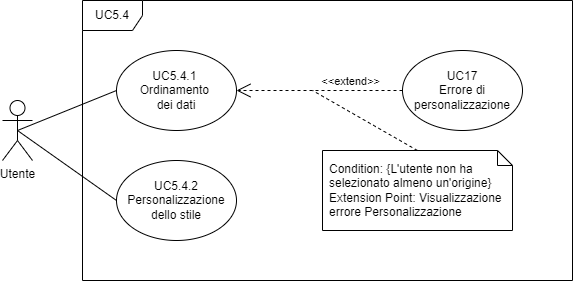
\includegraphics[scale=0.60]{../../assets/personalizzazioneSankey.png}
	\caption{UC5.4 - Personalizzazione $Sankey$ $Diagram^{G}$}
\end{figure}
\begin{itemize}
    \item \textbf{Attore primario:} Utente.
	\item \textbf{Precondizioni:} L'utente ha scelto il grafico $Sankey$ $Diagram^{G}$ \hyperref[sec:UC2.4]{UC2.4}.
	\item \textbf{Postcondizioni:} Il grafico viene ridisegnato secondo le scelte selezionate dall'utente.
	\item \textbf{Scenario principale:}L'utente decide:
	\begin{enumerate}
        \item Ordinamento dei dati \hyperref[sec:UC5.4.1]{UC5.4.1}.
        \item Personalizzazione dello stile \hyperref[sec:UC5.4.2]{UC5.4.2}.
    \end{enumerate}
\end{itemize}
\paragraph{UC5.4.1 - Ordinamento dei dati}
\label{sec:UC5.4.1}
    \begin{itemize}
        \item \textbf{Attore primario:} Utente.
        \item \textbf{Precondizioni:} L'utente ha selezionato $Sankey$ $Diagram^{G}$ \hyperref[sec:UC2.4]{UC2.4}.
	    \item \textbf{Postcondizioni:} L'utente ha deciso le ${\mathrm{dimensioni^{G}}}$ da rappresentare.
	    \item \textbf{Scenario principale:}
	    \begin{enumerate}
	    		\item L'utente sceglie i parametri per la rappresentazione dei rapporti tra i nodi.
		\end{enumerate}
	    \item \textbf{Estensioni:} Se non viene selezionata almeno un'origine tra i dati:
              \begin{itemize}
                  \item Non viene visualizzato nessun grafico.
                  \item Viene visualizzato un errore di personalizzazione grafico \hyperref[sec:UC17 - Errore di personalizzazione]{UC17}.
              \end{itemize}
    \end{itemize}
\paragraph{UC5.4.2 - Personalizzazione dello stile}
\label{sec:UC5.4.2}
\begin{itemize}
    \item \textbf{Attore primario:} Utente.
    \item \textbf{Precondizioni:} L'utente ha selezionato $Sankey$ $Diagram^{G}$ \hyperref[sec:UC2.4]{UC2.4}.
	\item \textbf{Postcondizioni:} L'utente ha selezionato i colori per le fasce del grafico.
	\item \textbf{Scenario principale:}
	\begin{enumerate}
		\item L'utente visualizza le opzioni di colori per la personalizzazione di ogni specifica del grafico.
		\item Nel caso l'utente non li modifichi rimangono quelli di default.
	\end{enumerate}
\end{itemize}

\newpage

% --------------------------------------------------------------------
% VISUALIZZAZIONE GRAFICO A TUTTO SCHERMO
% --------------------------------------------------------------------

\subsection{UC6 - Visualizzazione di un grafico a schermo intero}
\begin{figure}[h!]
	\centering
	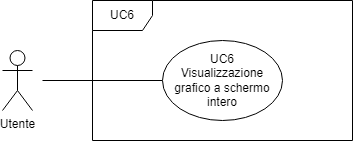
\includegraphics[scale=0.60]{../../assets/visualizzazione_fullscreen.png}
	\caption{UC6 - Visualizzazione di un grafico a schermo intero}
\end{figure}

\begin{itemize}
	\item \textbf{Attore primario:} Utente.
	\item \textbf{Precondizioni:} Il ${\mathrm{dataset^{G}}}$ è stato caricato correttamente. L'utente visualizza almeno un grafico sulla pagina. 
	\item \textbf{Postcondizioni:} 
	Viene mostrato il grafico scelto in \textit{fullscreen}.
	\item \textbf{Scenario principale:}
		\begin{enumerate}
			\item L'utente clicca sul pulsante di \textit{fullscreen} di un grafico.
			\item Il grafico viene visualizzato a schermo intero.
		\end{enumerate}
\end{itemize}
\newpage

% --------------------------------------------------------------------
% SEZIONE ZOOM INTERATTIVO
% --------------------------------------------------------------------

\subsection{UC7 - Zoom con selezione}
\label{sec:UC7}
\begin{figure}[h!]
    \centering
    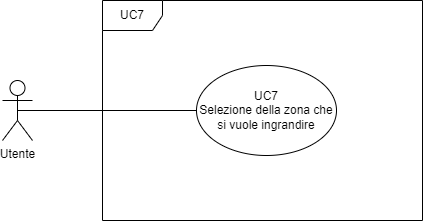
\includegraphics[scale=0.60]{../../assets/zoom_selezione.png}
    \caption{UC7 - Zoom con selezione sul grafico}
\end{figure}
\begin{itemize}
    \item \textbf{Attore primario}: Utente.
    \item \textbf{Precondizioni}: Il ${\mathrm{dataset^{G}}}$ è stato caricato correttamente. \par L'utente ha scelto la seguente tipologia di grafico:
    \begin{itemize}
    		\item $Scatter$ $Plot^{G}$.
    \end{itemize}
    \item \textbf{Postcondizioni}: Viene mostrato uno zoom della sezione selezionata dal mouse.
    \item \textbf{Scenario principale}:
          \begin{enumerate}
              \item L'utente seleziona con il mouse l'area all'interno del grafico che vuole ingrandire.
              \item L'area selezionata viene ingrandita.
          \end{enumerate}
\end{itemize}

\subsection{UC8 - Zoom con scroll del mouse}
\label{sec:UC8}
\begin{figure}[h!]
    \centering
    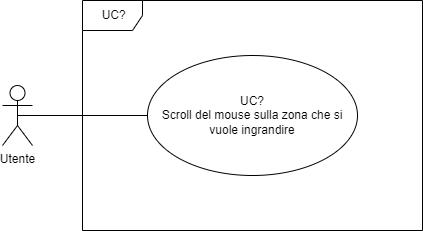
\includegraphics[scale=0.60]{../../assets/zoom_mouse.png}
    \caption{UC8 - Zoom con lo scroll del mouse}
\end{figure}
\begin{itemize}
    \item \textbf{Attore primario}: Utente.
    \item \textbf{Precondizioni}: Il ${\mathrm{dataset^{G}}}$ è stato caricato correttamente. \par L'utente ha scelto la seguente tipologia di grafico:
    \begin{itemize}
          \item $Force-directed$ $Graph^{G}$.
    \end{itemize}
    \item \textbf{Postcondizioni}: Viene mostrato uno zoom dove si trova il puntatore del mouse.
    \item \textbf{Scenario principale}:
          \begin{enumerate}
              \item L'utente posiziona il puntatore del mouse sulla zona di interesse.
              \item Per zoomare, l'utente esegue lo \textit{scroll} del mouse o utilizza le \textit{gesture} per lo zoom del \textit{trackpad}.
              \item L'area selezionata viene ingrandita.
          \end{enumerate}
\end{itemize}

\newpage

% --------------------------------------------------------------------
% SEZIONE MOUSE HOVER
% --------------------------------------------------------------------
\subsection{UC9 - Visualizzazione dettagli aggiuntivi}
\label{sec:UC9}
\begin{figure}[h!]
    \centering
    % Controlla che UC abbia il numero corretto
    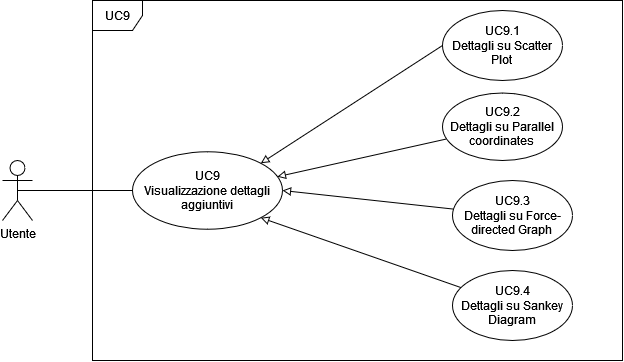
\includegraphics[scale=0.60]{../../assets/UC9-DettagliAggiuntivi.png}
    \caption{UC9 - Visualizzazione dettagli aggiuntivi}
\end{figure}
\begin{itemize}
    \item \textbf{Attore primario:} Utente.
    \item \textbf{Precondizioni:} Il ${\mathrm{dataset^{G}}}$ è stato caricato correttamente. L'utente ha scelto quale tipologia di grafico visualizzare e ha selezionato una vista$^{G}$.
    \item \textbf{Postcondizioni:} Vengono mostrate all'utente informazioni utili relative all'elemento su cui il mouse sta eseguendo l'hover.
    \item \textbf{Scenario principale}: 
    \begin{enumerate}
		\item L'utente passa con il mouse sopra ad un elemento di interesse. 
		\item Visualizza delle informazioni utili.
		\item L'elemento viene evidenziato. 
	\end{enumerate}
	Le tipologie di informazioni fornite dipendono dal grafico con cui l'utente interagisce, per questo vengono riportate le seguenti generalizzazioni.
    \item \textbf{Generalizzazioni:} \begin{enumerate}
                                        \item Dettagli aggiuntivi su \textit{$Scatter$ $Plot^{G}$} [\hyperref[sec:UC9.1]{UC9.1}]
                                        \item Dettagli aggiuntivi su \textit{$Parallel$ $Coordinates^{G}$} [\hyperref[sec:UC9.2]{UC9.2}]
                                        \item Dettagli aggiuntivi su \textit{$Force-directed$ $Graph^{G}$} [\hyperref[sec:UC9.3]{UC9.3}]
                                        \item Dettagli aggiuntivi su \textit{$Sankey$ $Diagram^{G}$} [\hyperref[sec:UC9.4]{UC9.4}]
                                    \end{enumerate}
\end{itemize}

\subsubsection{UC9.1 - Dettagli aggiuntivi su Scatter Plot}
\label{sec:UC9.1}
\begin{itemize}
    \item \textbf{Attore primario:} Utente.
    \item \textbf{Precondizioni:} Il ${\mathrm{dataset^{G}}}$ è stato caricato correttamente. L'utente ha scelto di visualizzare il grafico $Scatter$ $Plot^{G}$ e ha selezionato una vista$^{G}$.
    \item \textbf{Postcondizioni:} L'utente passando sopra con il mouse ad un punto sul grafico ottiene più informazioni relative a quel punto e lo evidenzia.
    \item \textbf{Scenario principale}: 
    \begin{enumerate}
		\item L'utente passa con il mouse sopra ad un punto sul grafico.
		\item Visualizza un'etichetta che contiene informazioni più complete relative a quel punto, come ad esempio: valore delle coordinate delle x, valore delle coordinate delle y. 
		\item Viene evidenziato il punto rispetto a tutti gli altri.
	\end{enumerate}
\end{itemize}

\subsubsection{UC9.2 - Dettagli aggiuntivi su Parallel Coordinates}
\label{sec:UC9.2}
\begin{itemize}
    \item \textbf{Attore primario:} Utente.
    \item \textbf{Precondizioni:} Il ${\mathrm{dataset^{G}}}$ è stato caricato correttamente. L'utente ha scelto di visualizzare il grafico $Parallel$ $Coordinates^{G}$ e ha selezionato una vista$^{G}$.
    \item \textbf{Postcondizioni:} L'utente passando sopra con il mouse a una linea, a un gruppo di linee o ad un asse ottiene maggiori informazioni a riguardo.
    \item \textbf{Scenario principale}:
    \begin{enumerate}
		\item L'utente passa con il mouse sopra ad una linea, ad un gruppo di linee o ad un asse sul grafico.
		\item Visualizza un'etichetta che contiene informazioni più complete relative a quella linea, a quel gruppo di linee o a quell'asse.
		\item Vengono evidenziati la linea, il gruppo intero o l'asse stesso.
	\end{enumerate}
\end{itemize}

\subsubsection{UC9.3 - Dettagli aggiuntivi su Force-directed Graph}
\label{sec:UC9.3}
\begin{itemize}
    \item \textbf{Attore primario:} Utente.
    \item \textbf{Precondizioni:} Il ${\mathrm{dataset^{G}}}$ è stato caricato correttamente. L'utente ha scelto di visualizzare il grafico $Force-directed$ $Graph^{G}$ e ha selezionato una vista$^{G}$.
    \item \textbf{Postcondizioni:} L'utente passando sopra con il mouse a un nodo del grafo lo evidenzia ed ottiene maggiori informazioni a riguardo.
    \item \textbf{Scenario principale}:
    \begin{enumerate}
		\item L'utente passa con il mouse sopra ad un nodo del grafo.
		\item Visualizza un \textit{tooltip} che mostra maggiori informazioni a riguardo. Ad esempio se un nodo rappresentasse il singolo tentativo di login, passandoci sopra con il mouse potrei visulizzare informazioni come l'ora in cui è avvenuto, l'indirizzo ip da cui si è verificato etc.
		\item Viene evidenziato il nodo.
	\end{enumerate}
\end{itemize}

\subsubsection{UC9.4 - Dettagli aggiuntivi su Sankey Diagram}
\label{sec:UC9.4}
\begin{itemize}
    \item \textbf{Attore primario:} Utente.
    \item \textbf{Precondizioni:} Il ${\mathrm{dataset^{G}}}$ è stato caricato correttamente. L'utente ha scelto di visualizzare il grafico $Sankey$ $Diagram^{G}$ e ha selezionato una vista$^{G}$.
    \item \textbf{Postcondizioni:} L'utente passando sopra con il mouse ad elemento nel grafico lo evidenzia.
    \item \textbf{Scenario principale}: 
    \begin{enumerate}
		\item L'utente passa con il mouse sopra ad un nodo del grafo.
		\item Vengono evidenziati il nodo ed i collegamenti da lui entranti e uscenti.
		\item L'utente passa con il mouse sopra ad un collegamento.
		\item Viene evidenziato il collegamento.
	\end{enumerate}
\end{itemize}

\newpage


% --------------------------------------------------------------------
% SEZIONE UC10 - DRAG DI UN NODO - FORCE DIRECTED
% --------------------------------------------------------------------
\subsection{UC10 - Drag di un nodo}
\label{sec:UC10}
\begin{figure}[h!]
    \centering
    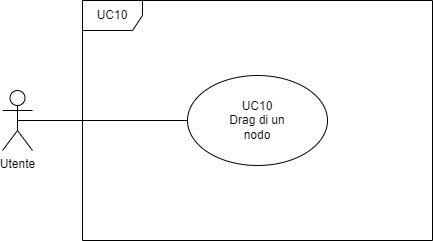
\includegraphics[scale=0.60]{../../assets/drag_nodo.png}
    \caption{UC10 - Drag di un nodo nel grafico $Force-directed$ $Graph^{G}$}
\end{figure}
\begin{itemize}
    \item \textbf{Attore primario}: Utente.
    \item \textbf{Precondizioni}: Il ${\mathrm{dataset^{G}}}$ è stato caricato correttamente. \par L'utente ha scelto la seguente tipologia di grafico:
    \begin{itemize}
    		\item $Force-directed$ $Graph^{G}$.
    \end{itemize}
    \item \textbf{Postcondizioni}: Il nodo viene trascinato secondo il movimento del mouse dell'utente.
    \item \textbf{Scenario principale}:
          \begin{enumerate}
              \item L'utente seleziona con il mouse il nodo da trascinare e lo clicca.
              \item Tenendo il nodo cliccato lo trascina a suo piacimento.
          \end{enumerate}
\end{itemize}

\newpage

% --------------------------------------------------------------------
% SEZIONE UC11 - CREAZIONE NUOVA VISTA
% --------------------------------------------------------------------
\subsection{UC11 - Creazione nuova vista}
\label{sec:UC11}
\begin{figure}[h!]
    \centering
    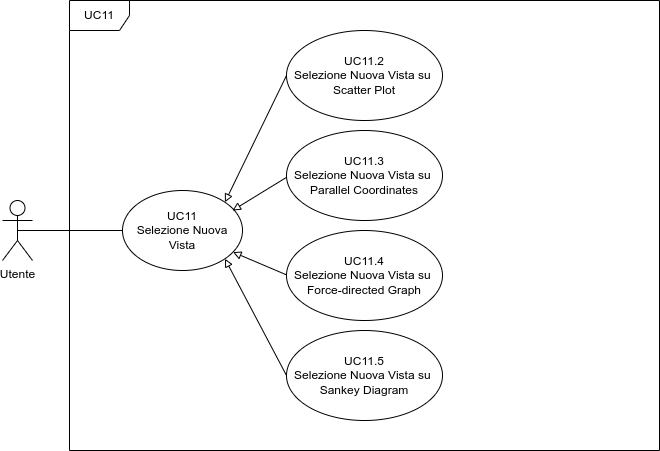
\includegraphics[scale=0.60]{../../assets/creazione_vista.png}
    \caption{UC11 - Creazione di una nuova vista$^{G}$}
\end{figure}
\begin{itemize}
    \item \textbf{Attore primario}: Utente.
    \item \textbf{Precondizioni}: Il ${\mathrm{dataset^{G}}}$ è stato caricato correttamente.
    \item \textbf{Postcondizioni}: L'utente ha creato una nuova vista$^{G}$ scegliendo quali colonne associare agli assi e quali righe visualizzare, oppure ha filtrato determinate celle da visualizzare.
    \item \textbf{Scenario principale}:
          \begin{enumerate}
              \item L'utente clicca il pulsante di creazione di una nuova vista$^{G}$.
              \item Il sistema visualizza la schermata di creazione.
              \item L'utente sceglie se selezionare tutte le colonne e righe del ${\mathrm{dataset^{G}}}$ o se selezionare solo determinate celle [\hyperref[sec:UC11.1]{UC11.1}].
              \item L'utente inserisce le informazioni richieste dalla schermata.
          \end{enumerate}
  \item \textbf{Generalizzazioni:} \begin{enumerate}
                                        \item Nuova vista$^{G}$ su $Scatter$ $Plot^{G}$ [\hyperref[sec:UC11.2]{UC11.2}]
                                        \item Nuova vista$^{G}$ su \textit{$Parallel$ $Coordinates^{G}$} [\hyperref[sec:UC11.3]{UC11.3}]
                                        \item Nuova vista$^{G}$ su \textit{$Force-directed$ $Graph^{G}$} [\hyperref[sec:UC11.4]{UC11.4}]
                                        \item Nuova vista$^{G}$ su \textit{$Sankey$ $Diagram^{G}$} [\hyperref[sec:UC11.5]{UC11.5}]
                                    \end{enumerate}
\end{itemize}

%Scelta colonne

\subsubsection{UC11.1 - Scelta delle colonne/righe/celle}
\label{sec:UC11.1}
\begin{itemize}
    \item \textbf{Attore primario:} Utente.
    \item \textbf{Precondizioni:} Il ${\mathrm{dataset^{G}}}$ è stato caricato correttamente. L'utente ha cliccato il pulsante ``Creazione nuova vista$^{G}$''.
    \item \textbf{Postcondizioni:} L'utente ha scelto quali righe e colonne utilizzare filtrando così le celle del ${\mathrm{dataset^{G}}}$ caricato.
    \item \textbf{Scenario principale}:
    \begin{enumerate}
		\item L'utente decide di creare una nuova vista$^{G}$.
		\item L'utente sceglie quali colonne, righe o multiple celle visualizzare.
		\item L'utente può anche scegliere di selezionarle tutte.
	\end{enumerate}
	\item \textbf{Estensioni:} Nel caso in cui l'utente non abbia selezionato un numero sufficiente di celle o non ne abbia selezionata alcuna:
              \begin{itemize}
                  \item Non viene visualizzato nessun grafico.
                  \item Viene visualizzato un errore di scelta celle insufficienti \hyperref[sec:UC19 - Errore-celle-insufficienti]{UC19}.
              \end{itemize}
\end{itemize}


%Scatter Plot

\subsubsection{UC11.2 - Nuova vista su Scatter Plot}
\label{sec:UC11.2}
\begin{figure}[h!]
	\centering
	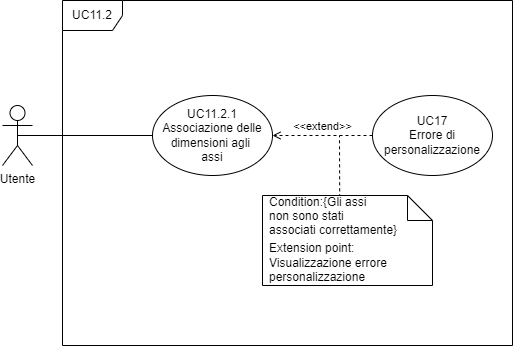
\includegraphics[scale=0.60]{../../assets/creazionevista_scatter_plot.png}
	\caption{UC11.2 - Nuova vista$^{G}$ su $Scatter$ $Plot^{G}$}
\end{figure}
\begin{itemize}
    \item \textbf{Attore primario:} Utente.
    \item \textbf{Precondizioni:} Il ${\mathrm{dataset^{G}}}$ è stato caricato correttamente. L'utente ha cliccato il pulsante ``Creazione nuova vista$^{G}$'' scegliendo quali celle/righe/colonne visualizzare (\hyperref[sec:UC11.1]{UC11.1}) e ha scelto il grafico Scatter Plot.
    \item \textbf{Postcondizioni:} Il grafico viene mostrato secondo le scelte selezionate dall'utente.
    \item \textbf{Scenario principale}:
    \begin{enumerate}
		\item L'utente decide di creare una nuova vista$^{G}$ per il grafico $Scatter$ $Plot^{G}$.
		\item L'utente può dunque associare le ${\mathrm{dimensioni^{G}}}$ desiderate agli assi del grafico. \hyperref[sec:UC11.2.1]{UC11.2.1}.
	\end{enumerate}
\end{itemize}

\paragraph{UC11.2.1 - Associazione delle dimensioni agli assi}
\label{sec:UC11.2.1}
    \begin{itemize}
        \item \textbf{Attore primario:} Utente.
        \item \textbf{Precondizioni:} Valgono le precondizioni di \hyperref[sec:UC11.2]{UC11.2}.
	    \item \textbf{Postcondizioni:} L'utente ha associato le ${\mathrm{dimensioni^{G}}}$ disponibili con gli assi del grafico.
	    \item \textbf{Scenario principale:} 
	    \begin{enumerate}
	    		\item L'utente sceglie quali dimensioni$^{G}$ associare agli assi del grafico.
		\end{enumerate}
	    \item \textbf{Estensioni:} Nel caso l'utente non abbia associato correttamente le ${\mathrm{dimensioni^{G}}}$ agli assi del grafico:
              \begin{itemize}
                  \item Non viene visualizzato nessun grafico.
                  \item Viene visualizzato un errore di personalizzazione grafico \hyperref[sec:UC17 - Errore di personalizzazione]{UC17}.
              \end{itemize}
    \end{itemize}

\newpage
%Parallel Coordinates

\subsubsection{UC11.3 - Nuova vista su Parallel Coordinates}
\label{sec:UC11.3}
\begin{figure}[h!]
	\centering
	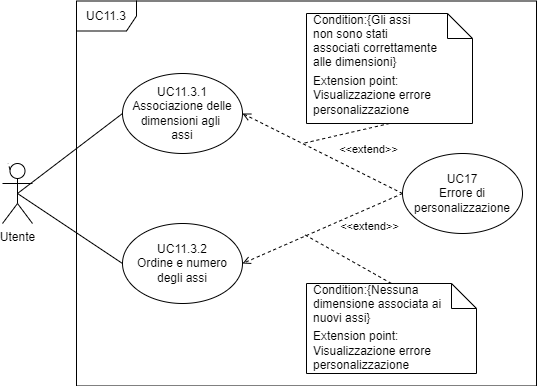
\includegraphics[scale=0.60]{../../assets/creazionevista_parallel_coordinates.png}
	\caption{UC11.3 - Nuova vista$^{G}$ su $Parallel$ $Coordinates^{G}$}
\end{figure}
\begin{itemize}
    \item \textbf{Attore primario:} Utente.
    \item \textbf{Precondizioni:} Il ${\mathrm{dataset^{G}}}$ è stato caricato correttamente. L'utente ha cliccato il pulsante ``Creazione nuova vista$^{G}$'' scegliendo quali celle/righe/colonne visualizzare (\hyperref[sec:UC11.1]{UC11.1}) e ha scelto il grafico $Parallel$ $Coordinates^{G}$.
    \item \textbf{Postcondizioni:} Il grafico viene mostrato secondo le scelte selezionate dall'utente.
    \item \textbf{Scenario principale}:
    \begin{enumerate}
		\item L'utente decide di creare una nuova vista$^{G}$ per il grafico $Parallel$ $Coordinates^{G}$.
		\item L'utente può associare le ${\mathrm{dimensioni^{G}}}$ desiderate agli assi \hyperref[sec:UC11.3.1]{UC11.3.1}.
		\item L'utente può decidere ordine e numero degli assi \hyperref[sec:UC11.3.2]{UC11.3.2}.
		\item L'utente può decidere lo \textit{scaling} dei dati \hyperref[sec:UC11.3.3]{UC11.3.3}.
	\end{enumerate}
\end{itemize}

\paragraph{UC11.3.1 - Associazione delle dimensioni agli assi}
\label{sec:UC11.3.1}
    \begin{itemize}
        \item \textbf{Attore primario:} Utente.
        \item \textbf{Precondizioni:} Valgono le precondizioni di \hyperref[sec:UC11.3]{UC11.3}.
	    \item \textbf{Postcondizioni:} L'utente ha associato le ${\mathrm{dimensioni^{G}}}$ disponibili agli assi del grafico.
	    \item \textbf{Scenario principale:} 
	    \begin{enumerate}
	    		\item L'utente sceglie quali colonne associare agli assi del grafico.
		\end{enumerate}
	    \item \textbf{Estensioni:} Nel caso l'utente non abbia associato correttamente gli assi del grafico:
              \begin{itemize}
                  \item Non viene visualizzato nessun grafico.
                  \item Viene visualizzato un errore di personalizzazione grafico \hyperref[sec:UC17 - Errore di personalizzazione]{UC17}.
              \end{itemize}
    \end{itemize}
    
\paragraph{UC11.3.2 - Ordine e numero degli assi}
\label{sec:UC11.3.2}
    \begin{itemize}
        \item \textbf{Attore primario:} Utente.
        \item \textbf{Precondizioni:} Valgono le precondizioni di \hyperref[sec:UC11.3]{UC11.3}.
	    \item \textbf{Postcondizioni:} L'utente ha modificato l'ordine verticale degli assi e il numero.
	    \item \textbf{Scenario principale:} 
	    \begin{enumerate}
	    		\item L'utente sceglie ordine e numero degli assi.
		\end{enumerate}
	    \item \textbf{Estensioni:} Nel caso l'utente abbia creato nuovi assi ma non abbia associato nessuna ${\mathrm{dimen^{G}}}$ ad essi:
              \begin{itemize}
                  \item Non viene visualizzato nessun grafico.
                  \item Viene visualizzato un errore di visualizzazione personalizzazione grafico \hyperref[sec:UC17 - Errore di personalizzazione]{UC17}.
              \end{itemize}
    \end{itemize}
    
\paragraph{UC11.3.3 - Scaling dei dati}
\label{sec:UC11.3.3}
    \begin{itemize}
        \item \textbf{Attore primario:} Utente.
        \item \textbf{Precondizioni:} Valgono le precondizioni di \hyperref[sec:UC11.3]{UC11.3}.
	    \item \textbf{Postcondizioni:} L'utente ha ridimensionato i dati in una nuova scala comune tra le variabili o viceversa.
	    \item \textbf{Scenario principale:} 
	    \begin{enumerate}
	    		\item L'utente sceglie lo \textit{scaling} dei dati.
		\end{enumerate}
    \end{itemize}

\newpage
%Force-directed

\subsubsection{UC11.4 - Nuova vista su Force-directed Graph}
\label{sec:UC11.4}
\begin{figure}[h!]
	\centering
	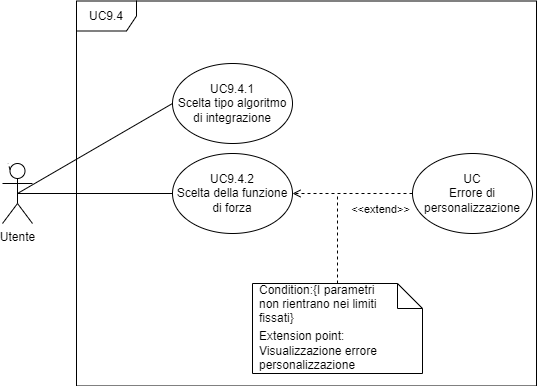
\includegraphics[scale=0.60]{../../assets/creazionevista_force.png}
	\caption{UC11.4 - Nuova vista$^{G}$ su $Force-directed$ $Graph^{G}$}
\end{figure}
\begin{itemize}
    \item \textbf{Attore primario:} Utente.
    \item \textbf{Precondizioni:} Il ${\mathrm{dataset^{G}}}$ è stato caricato correttamente. L'utente ha cliccato il pulsante ``Creazione nuova vista$^{G}$'' scegliendo quali celle/righe/colonne visualizzare (\hyperref[sec:UC11.1]{UC11.1}) e ha scelto il grafico $Force-directed Graph^{G}$.
    \item \textbf{Postcondizioni:} Il grafico viene mostrato secondo le scelte selezionate dall'utente.
    \item \textbf{Scenario principale}:
    \begin{enumerate}
		\item L'utente decide di creare una nuova vista$^{G}$ per il grafico $Force-directed$ $Graph^{G}$.
		\item L'utente può decidere un algoritmo di integrazione \hyperref[sec:UC11.4.1]{UC11.4.1}.
		\item L'utente può decidere la funzione di forza \hyperref[sec:UC11.4.2]{UC11.4.2}.
	\end{enumerate}
\end{itemize}

\paragraph{UC11.4.1 - Scelta algoritmo di integrazione}
\label{sec:UC11.4.1}
    \begin{itemize}
        \item \textbf{Attore primario:} Utente.
        \item \textbf{Precondizioni:} Valgono le precondizioni di \hyperref[sec:UC11.4]{UC11.4}.
	    \item \textbf{Postcondizioni:} L'utente ha associato l'algoritmo di integrazione che desidera.
	    \item \textbf{Scenario principale:} 
	    \begin{enumerate}
	    		\item L'utente sceglie l'algoritmo di integrazione.
		\end{enumerate}
    \end{itemize}
    
\paragraph{UC11.4.2 - Scelta funzione di forza}
\label{sec:UC11.4.2}
    \begin{itemize}
        \item \textbf{Attore primario:} Utente.
        \item \textbf{Precondizioni:} Valgono le precondizioni di \hyperref[sec:UC11.4]{UC11.4}.
	    \item \textbf{Postcondizioni:} L'utente ha deciso la funzione di forza tra i nodi.
	    \item \textbf{Scenario principale:} 
	    \begin{enumerate}
	    		\item L'utente sceglie i parametri per la rappresentazione dei rapporti tra i nodi.
		\end{enumerate}
	    \item \textbf{Estensioni:} Nel caso l'utente abbia selezionato dei parametri che non rientrino nei limiti fissati:
              \begin{itemize}
                  \item Non viene visualizzato nessun grafico.
                  \item Viene visualizzato un errore di visualizzazione personalizzazione grafico \hyperref[sec:UC17 - Errore di personalizzazione]{UC17}.
              \end{itemize}
    \end{itemize}


%Sankey

\subsubsection{UC11.5 - Nuova vista su Sankey Diagram}
\label{sec:UC11.5}
\begin{figure}[h!]
	\centering
	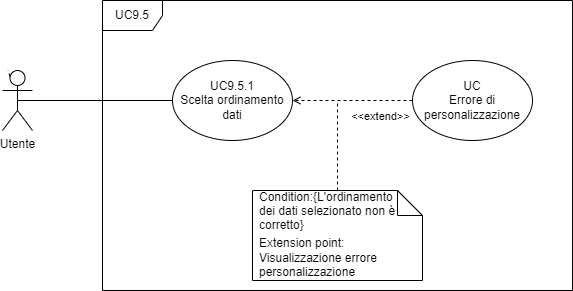
\includegraphics[scale=0.60]{../../assets/creazionevista_sankey.png}
	\caption{UC11.5 - Nuova vista$^{G}$ su $Sankey$ $Diagram^{G}$}
\end{figure}
\begin{itemize}
    \item \textbf{Attore primario:} Utente.
    \item \textbf{Precondizioni:} Il ${\mathrm{dataset^{G}}}$ è stato caricato correttamente. L'utente ha cliccato il pulsante ``Creazione nuova vista$^{G}$'' scegliendo quali celle/righe/colonne visualizzare (\hyperref[sec:UC11.1]{UC11.1}) e ha scelto il grafico Sankey Diagram.
    \item \textbf{Postcondizioni:} Il grafico viene mostrato secondo le scelte selezionate dall'utente.
    \item \textbf{Scenario principale}:
    \begin{enumerate}
		\item L'utente decide di creare una nuova vista$^{G}$ per il grafico $Sankey$ $Diagram^{G}$.
		\item L'utente può decidere un ordinamento dei dati \hyperref[sec:UC11.5.1]{UC11.5.1}.
	\end{enumerate}
\end{itemize}

\paragraph{UC11.5.1 - Scelta ordinamento dei dati}
\label{sec:UC11.5.1}
    \begin{itemize}
        \item \textbf{Attore primario:} Utente.
        \item \textbf{Precondizioni:} Valgono le precondizioni di \hyperref[sec:UC11.5]{UC11.5}.
	    \item \textbf{Postcondizioni:} L'utente ha stabilito le ${\mathrm{dimensioni^{G}}}$ da rappresentare.
	    \item \textbf{Scenario principale:}
	    \begin{enumerate}
	    		\item L'utente sceglie l'ordinamento dei dati.
		\end{enumerate}
		\item \textbf{Estensioni:} Se non viene selezionata almeno un'origine nei dati:
              \begin{itemize}
                  \item Non viene visualizzato nessun grafico.
                  \item Viene visualizzato un errore di visualizzazione personalizzazione grafico \hyperref[sec:UC17 - Errore di personalizzazione]{UC17}.
              \end{itemize}
    \end{itemize}


\newpage
% --------------------------------------------------------------------
% SEZIONE SALVATAGGIO VISTA SU FILE
% --------------------------------------------------------------------

\subsection{UC12 - Salvataggio vista}
\label{sec:UC12}
\begin{figure}[h!]
    \centering
    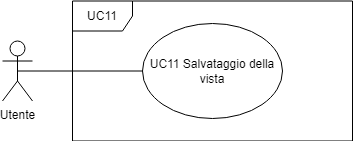
\includegraphics[scale=0.60]{../../assets/salvataggio_vista.png}
    \caption{UC12 - Salvataggio della vista$^{G}$ su file}
\end{figure}
\begin{itemize}
    \item \textbf{Attore primario}: Utente.
    \item \textbf{Precondizioni}: Il ${\mathrm{dataset^{G}}}$ è stato caricato correttamente. L'utente ha scelto una tipologia di grafico e ha creato una propria vista$^{G}$ personalizzata.
    \item \textbf{Postcondizioni}: La vista$^{G}$ viene salvata all'interno di un file ${\mathrm{.json^{G}}}$.
    \item \textbf{Scenario principale}:
          \begin{enumerate}
              \item L'utente seleziona il pulsante di salvataggio della vista$^{G}$.
              \item Il file viene scaricato in locale in formato ${\mathrm{.json^{G}}}$.
          \end{enumerate}
\end{itemize}

\newpage

% --------------------------------------------------------------------
% SEZIONE CARICAMENTO VISTA
% --------------------------------------------------------------------

\subsection{UC13 - Caricamento vista}
\label{sec:UC13}
\begin{figure}[h!]
    \centering
    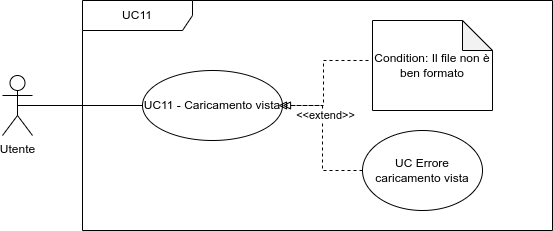
\includegraphics[scale=0.60]{../../assets/caricamento_vista.png}
    \caption{UC13 - Caricamento della vista$^{G}$ da file}
\end{figure}
\begin{itemize}
    \item \textbf{Attore primario}: Utente.
    \item \textbf{Precondizioni}: Il ${\mathrm{dataset^{G}}}$ è stato caricato correttamente.
    \item \textbf{Postcondizioni}: È selezionabile la nuova vista$^{G}$ nel menù viste$^{G}$ descritto da \hyperref[sec:UC3]{UC3}.
    \item \textbf{Scenario principale}:
          \begin{enumerate}
              \item L'utente preme il pulsante "carica vista$^{G}$".
              \item L'utente seleziona il file ${\mathrm{.json^{G}}}$ contenente la vista$^{G}$.
              \item L'applicativo rende disponibile la vista$^{G}$ appena caricata.
          \end{enumerate}
    \item \textbf{Estensioni:}
    \begin{itemize}
        \item Nel caso il ${\mathrm{.json^{G}}}$ contenente la vista$^{G}$ non sia ben formato: 
        \begin{enumerate}
            \item La vista$^{G}$ non viene caricata.
            \item Viene visualizzato un messaggio d'errore. [\hyperref[sec:UC18 - Errore caricamento vista]{UC18}]
        \end{enumerate}
    \end{itemize}
\end{itemize}

\newpage

% --------------------------------------------------------------------
% SEZIONE ERRORI
% --------------------------------------------------------------------

\section{Errori}
\subsection{UC14 - Errore formato file}
\label{sec:UC14 - Errore formato file}
\begin{itemize}
    \item \textbf{Attore primario:} Utente
    \item \textbf{Precondizioni:} L'utente carica un file in un formato non supportato.
    \item \textbf{Postcondizioni:} L'utente visualizza un messaggio di errore e il file non viene caricato.
    \item \textbf{Scenario principale:}
          \begin{enumerate}
              \item L'utente visualizza un messaggio di errore esplicativo
              \item L'utente clicca "OK" per proseguire.
          \end{enumerate}
\end{itemize}

\subsection{UC15 - Errore struttura dataset}
\label{sec:UC15 - Errore struttura dataset}
\begin{itemize}
    \item \textbf{Attore primario:} Utente
    \item \textbf{Precondizioni:} L'utente carica un file nel formato supportato ma che non è correttamente strutturato  
                                  (e.g. due o più colonne sono invertite oppure una o più colonne sono mancanti). 
    \item \textbf{Postcondizioni:} L'utente visualizza un messaggio di errore e il file non viene caricato.
    \item \textbf{Scenario principale:}
          \begin{enumerate}
              \item L'utente visualizza un messaggio di errore esplicativo.
              \item L'utente clicca "OK" per proseguire.
          \end{enumerate} 
\end{itemize}

\subsection{UC16 - Errore validità riga nel dataset}
\label{sec:UC16 - Errore validità riga}
\begin{itemize}
    \item \textbf{Attore primario:} Utente
    \item \textbf{Precondizioni:} L'utente carica un file nel formato supportato e ben strutturato ma una o più righe presentano un dato non valido (e.g. nella colonna relativa ai \textit{timestamp} il valore è negativo).  
    \item \textbf{Postcondizioni:} L'utente visualizza un messaggio di errore che chiede se ignorare la riga non valida, oppure continuare.
    \item \textbf{Scenario principale:}
    \begin{itemize}
        \item   L'utente sceglie di ignorare la riga:
                \begin{enumerate}
                    \item L'utente visualizza un messaggio di errore esplicativo.
                    \item L'utente clicca "IGNORA" per ignorare la riga non valida.
                    \item Il file viene caricato escludendo la riga precedentemente ignorata.
                \end{enumerate} 
        \item   L'utente sceglie di proseguire:
                \begin{enumerate}
                    \item L'utente visualizza un messaggio di errore esplicativo.
                    \item L'utente clicca "OK" per proseguire.
                    \item Il file non viene caricato.
                \end{enumerate} 
    \end{itemize}
\end{itemize}

\subsection{UC17 - Errore di personalizzazione grafico}
\label{sec:UC17 - Errore di personalizzazione}
\begin{itemize}
    \item \textbf{Attore primario:} Utente
    \item \textbf{Precondizioni:}
    		\begin{itemize}
    			\item L'utente associa non correttamente una o più ${\mathrm{dimensioni^{G}}}$ ad uno o più assi nel grafico.
    			\item L'utente inserisce dei parametri relativi alla funzione di forza non corretti.
    			\item L'utente sceglie dei parametri relativi all'ordinamento dei dati non corretti.
    		\end{itemize}
    \item \textbf{Postcondizioni:} L'utente visualizza un messaggio d'errore esplicativo relativo alla condizione che ha causato l'errore, e le modifiche da lui apportate non vengono eseguite.
    \item \textbf{Scenario principale:}
    \begin{enumerate}
        \item L'utente visualizza un messaggio di errore esplicativo.
        \item L'utente clicca "OK" per proseguire.
    \end{enumerate}
\end{itemize}

\subsection{UC18 - Errore caricamento vista}
\label{sec:UC18 - Errore caricamento vista}
\begin{itemize}
    \item \textbf{Attore primario:} Utente
    \item \textbf{Precondizioni:} L'utente carica un file vista$^{G}$ malformato.
    \item \textbf{Postcondizioni:} L'utente visualizza un messaggio d'errore esplicativo relativo alla condizione che ha causato l'errore, non viene caricata la vista$^{G}$.
    \item \textbf{Scenario principale:}
    \begin{enumerate}
        \item L'utente visualizza un messaggio di errore esplicativo.
        \item L'utente clicca "OK" per proseguire.
    \end{enumerate}
\end{itemize}

\subsection{UC19 - Errore scelta celle insufficienti}
\label{sec:UC19 - Errore-celle-insufficienti}
\begin{itemize}
    \item \textbf{Attore primario:} Utente
    \item \textbf{Precondizioni:} Il ${\mathrm{dataset^{G}}}$ è stato caricato correttamente. L'utente ha cliccato il pulsante ``Creazione nuova vista$^{G}$'' e ha inserito le colonne/righe/celle che vuole utilizzare (\hyperref[sec:UC9.1]{UC9.1}).
    \item \textbf{Postcondizioni:} L'utente visualizza un messaggio di errore per celle insufficienti. 
    \item \textbf{Scenario principale:}
          \begin{enumerate}
              \item L'utente ha selezionato un numero di celle insufficienti o nessuna.
              \item Viene visualizzato un messaggio di errore.
              \item L'utente clicca "OK" per proseguire.
          \end{enumerate} 
\end{itemize}

